\chapter{الفئة p \texorpdfstring{\babelsublr{(1)}}{(1)}: زمر البور والكربون والنيتروجين}\label{ch:b1:p-block-13-15}

الهواء الذي نتنفسه أربعة أخماسه نيتروجين، ومع ذلك تجوع النباتات إليه:
فالرابطة الثلاثية \ce{N#N} بالغة القوة إلى حد أن شيئًا لا يكاد يكسرها. وطوال
معظم التاريخ، جاء نيتروجين المحاصيل من السماد الحيواني، ومن بكتيريا تعيش
على جذور البقوليات، ومن النترات المستخرجة من المناجم. وفي مطلع القرن
العشرين غيّر ذلك تفاعلٌ بين النيتروجين والهيدروجين على \omterm{def:b1:elementary-steps:catalyst}{حفّاز} من الحديد؛
واليوم يصنع العالم نحو 160 مليون طن من النيتروجين
سنويًا على هيئة أمونيا، ونحو نصف النيتروجين في جسم الإنسان
مرّ عبر مصنع للأمونيا. والزمر 13 و14 و15 تضم عناصر
تلك القصة --- النيتروجين والفوسفور للأسمدة، والكربون
والسيليكون للحياة والصخور، والبور والألومنيوم للزجاج والسبائك
الخفيفة. يستعرضها هذا الفصل بأدوات الفصول السابقة.

\begin{recall}
\omterm{def:b1:crystals-metals:allotropy}{متآصلات} الكربون وبنية السيليكون والسيليكا
(\cref{ch:b1:crystals-ionic-covalent})؛ وطابع الأكاسيد
(\cref{def:b1:s-block:oxide-character})؛ \omterm{def:b1:nernst:oxidation-number}{وأعداد الأكسدة} \omterm{def:b1:nernst:electrode-potential}{والجهود
المعيارية} (\cref{ch:b1:nernst})؛ \omterm{def:b1:precipitation:amphoteric-hydroxide}{والهيدروكسيدات المذبذبة}
(\cref{ch:b1:precipitation})؛ وثوابت التوازن من طاقات جيبس
(\cref{ch:b1:extent-q-and-k}).
\end{recall}
% ledger: usgs:N-world-2025

\begin{omfigure}
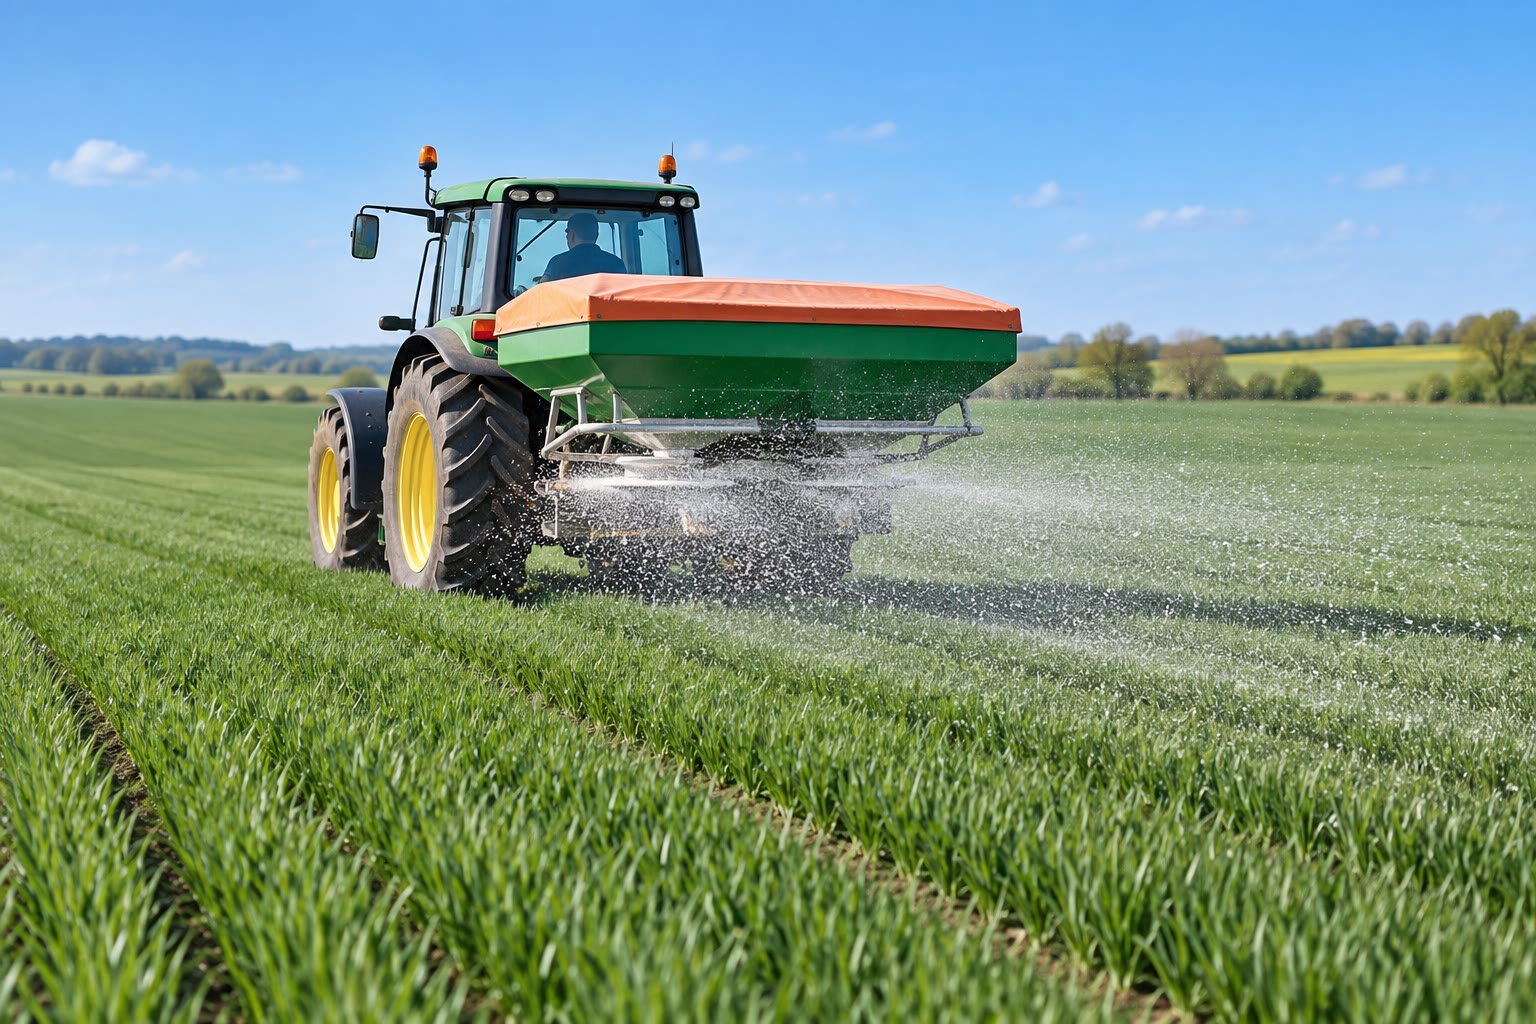
\includegraphics[width=0.55\linewidth]{images/book2/ai/b1-27-fertiliser-field.jpg}

{\small نثر سماد نيتروجيني على حقل قمح. وقد صُنع معظمه
من نيتروجين الهواء بطريقة هابر--بوش.}
\end{omfigure}

\section{الزمرة 13: البور والألومنيوم}

البور \omterm{def:b1:periodicity:metalloid}{شبه فلز} يكوّن مركبات تساهمية ثمانيتها
ناقصة: ففي \ce{BF3} وحمض البوريك \ce{B(OH)3} للبور ستة \omterm{def:b1:quantum-numbers:configuration}{إلكترونات
تكافؤ} ويسلك سلوك \omterm{def:b1:lewis-resonance-vsepr:lewis-acid}{حمض لويس} (\cref{ch:b1:lewis-resonance-vsepr}).
وحمض البوريك \omterm{def:b1:predominant-reaction:strong-acid}{حمض ضعيف} لا بفقد بروتون بل باستقبال
أيون هيدروكسيد، \ce{B(OH)3 + 2H2O <=> B(OH)4- + H3O+}. والبوراكس، وهو بورات
صوديوم، يُستعمل في الزجاج والمنظفات.

\begin{definition}[الحمض الأكسجيني]\label{def:b1:p-block-13-15:oxoacid}
\emph{الحمض الأكسجيني}\index{حمض أكسجيني} حمض تكون فيه ذرات الهيدروجين
الحمضية مرتبطة بذرات أكسجين مرتبطة \omterm{def:b1:complexation:complex}{بذرة مركزية}:
\ce{B(OH)3}، \ce{H2CO3}، \ce{HNO3} (\ce{HO-NO2})، \ce{H3PO4}
(\ce{(HO)3PO})، \ce{H2SO4}. وكلما كثرت ذرات الأكسجين غير الحاملة للهيدروجين حول
\omterm{def:b1:complexation:complex}{الذرة المركزية}، كان الحمض أقوى.
\end{definition}

الألومنيوم، الواقع تحت البور، فلز، لكن أيونه الصغير العالي الشحنة
يمنحه أكسيدًا وهيدروكسيدًا مذبذبين (\cref{sec:b1:precipitation:amphoteric}).
وخامه البوكسيت، وهو خليط من هيدروكسيدات الألومنيوم مع أكاسيد الحديد
والسيليكا؛ وفي سنة 2025 استخرج العالم نحو 440 مليون طن من البوكسيت
وكرّر منه نحو 150 مليون طن من الألومينا.
% ledger: usgs:bauxite-world-2025, usgs:alumina-world-2025

\begin{proposition}[طريقة باير]\label{prop:b1:p-block-13-15:bayer}
يذيب هيدروكسيد الصوديوم المركّز الساخن ألومنيوم البوكسيت على هيئة
\ce{Al(OH)4-} ويترك أكاسيد الحديد (الطين الأحمر)؛ ويُرسّب تبريد المحلول المرشَّح
وتلقيحه \ce{Al(OH)3} نقيًا، يُكلَّس إلى ألومينا،
\ce{2Al(OH)3 -> Al2O3 + 3H2O}.
\end{proposition}

\begin{proof}
للتفاعل \ce{Al(OH)3(s) + OH- <=> Al(OH)4-} الثابت $K = 10^{-1.23}$ عند
\qty{25}{\celsius} (\cref{ch:b1:precipitation}): فعند \ce{[OH-]} مرتفع يكون
الألومنيوم في المحلول، بينما يبقى هيدروكسيد الحديد(III)، غير المذبذب،
صلبًا (\cref{exo:b1:precipitation:12}). ويخفض التخفيف والتبريد
\ce{[OH-]} ويزيحان حاصل التفاعل بحيث يصير $Q > K$ للتفاعل
العكسي: فيترسب الهيدروكسيد. ويزيل التكليس الماء.
\end{proof}

ثم تُختزل الألومينا إلى ألومنيوم بالتحليل الكهربائي في الكريوليت المنصهر،
وهي صناعة تُدرس في مجلد السنة الثانية.

\begin{omfigure}
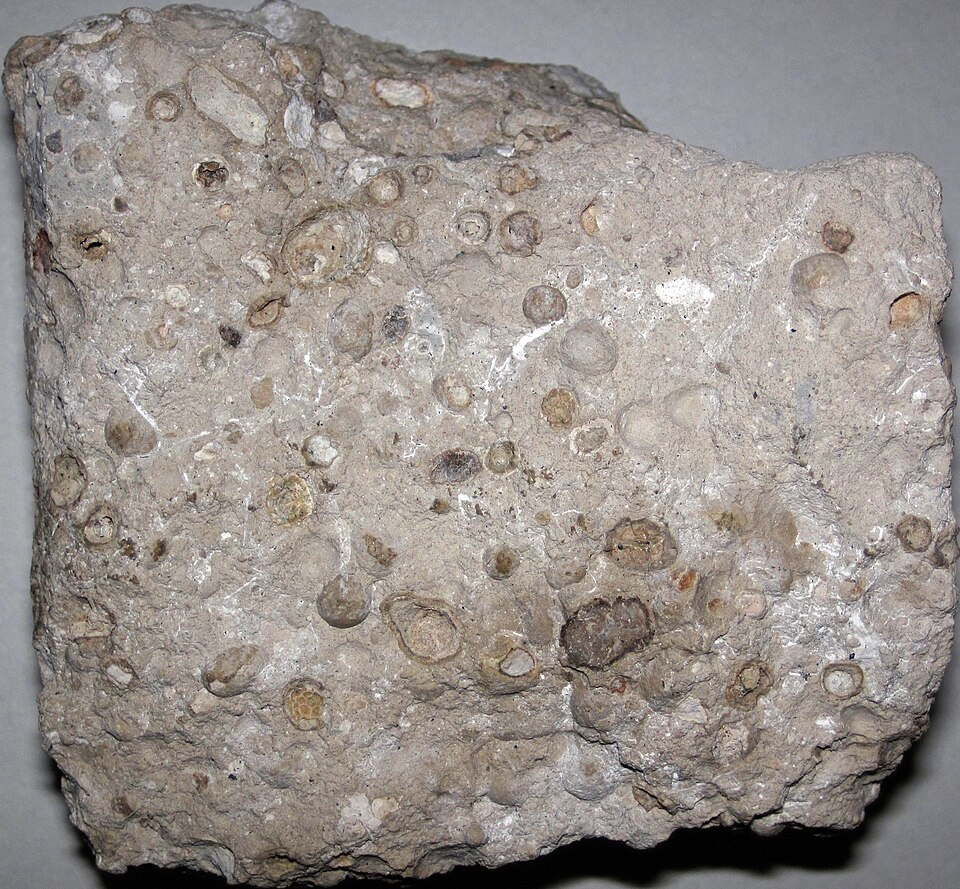
\includegraphics[height=3.6cm]{images/book2/bauxite.jpg}\hspace{0.4em}%
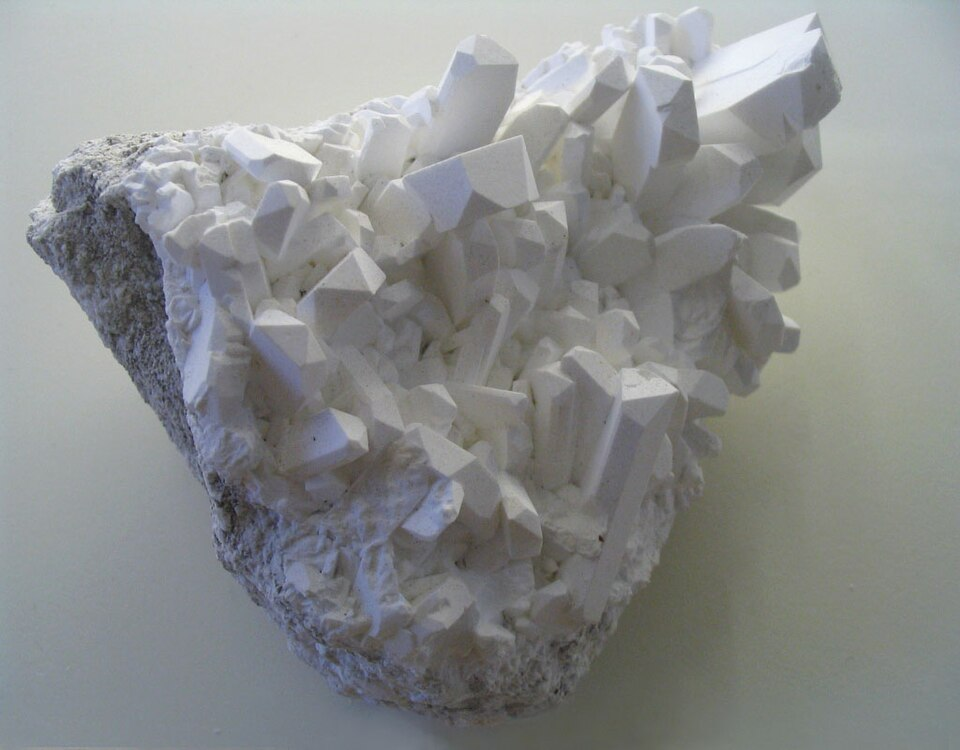
\includegraphics[height=3.6cm]{images/book2/borax.jpg}\hspace{0.4em}%
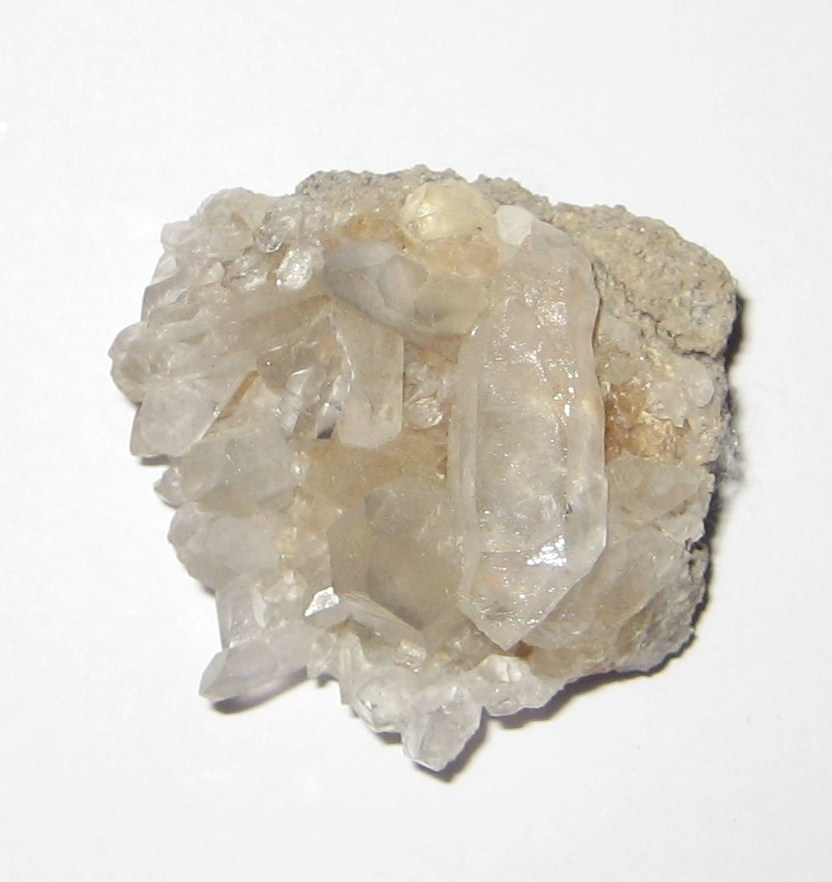
\includegraphics[height=3.6cm]{images/book2/quartz.jpg}\hspace{0.4em}%
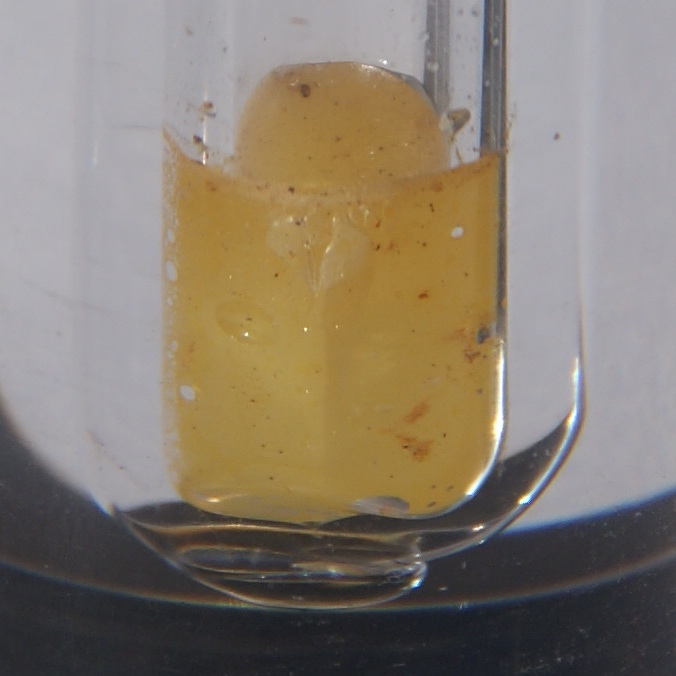
\includegraphics[height=3.6cm]{images/book2/white-phosphorus.jpg}

{\small من اليمين إلى اليسار: بوكسيت حمّصي (جيمس سانت جون، CC BY 2.0)؛
بلورات البوراكس (آرام دوليان، ملكية عامة)؛ عنقود من بلورات الكوارتز،
\ce{SiO2} (ستيفاني كليفورد، CC BY 2.0)؛ الفوسفور الأبيض، مع قليل من
الفوسفور الأحمر، محفوظ تحت الماء لأنه يشتعل في الهواء (صور عالية الدقة
للعناصر الكيميائية، CC BY 3.0). كلها من ويكيميديا كومنز.}
\end{omfigure}

\section{الزمرة 14: الكربون والسيليكون}

يكوّن الكربون والسيليكون كلاهما أربع روابط، لكن بطريقتين مختلفتين. فالكربون يكوّن
روابط ثنائية قوية: \ce{CO2} جزيء، \ce{O=C=O}، وهو غاز. أما السيليكون
فلا يكاد يفعل ذلك: \ce{SiO2} شبكة تساهمية من رباعيات أوجه \ce{SiO4}
تتقاسم رؤوسها كلها، وهو صلب قاسٍ، الكوارتز (\cref{ch:b1:crystals-ionic-covalent}).
وثنائي أكسيد الكربون \omterm{def:b1:s-block:oxide-character}{أكسيد حمضي}، يعطي حمض الكربونيك، والهيدروجين كربونات
والكربونات (\cref{ch:b1:predominant-reaction})؛ والسيليكا \omterm{def:b1:s-block:oxide-character}{أكسيد
حمضي} أيضًا، تهاجمه القلويات المنصهرة فتعطي سيليكات.

\begin{proposition}[وحدات السيليكات]\label{prop:b1:p-block-13-15:silicate-units}
تُبنى السيليكات من رباعيات أوجه \ce{SiO4}؛ وعدد الرؤوس المتقاسمة
مع رباعيات أوجه أخرى يحدد صيغة الأنيون: لا شيء، \ce{SiO4^4-}
(رباعيات أوجه معزولة)؛ اثنان، سلاسل $(\ce{SiO3})_n^{2n-}$؛ ثلاثة، صفائح
$(\ce{Si2O5})_n^{2n-}$؛ أربعة، الهيكل المتعادل \ce{SiO2}.
\end{proposition}

\begin{proof}
ذرة الأكسجين المتقاسمة ينتمي نصفها إلى كل رباعي أوجه. ورباعي الأوجه الذي يتقاسم
$k$ رأسًا يملك $4 - k$ ذرة أكسجين ملكًا تامًا و$k$ بالنصف: أي $4 -
k/2$ ذرة أكسجين لكل ذرة سيليكون. وكل ذرة أكسجين غير متقاسمة تحمل شحنة $-1$ (إذ
لها رابطة واحدة)، والمتقاسمة لا شحنة لها: فالشحنة لكل ذرة سيليكون
$-(4 - k)$. $k = 0$: \ce{SiO4^4-}؛ $k = 2$: \ce{SiO3^2-} لكل ذرة سيليكون؛
$k = 3$: \ce{SiO_{2.5}^-}، أي \ce{Si2O5^2-}؛ $k = 4$: \ce{SiO2}.
\end{proof}

\begin{omfigure}
\begin{tikzpicture}[font=\small, line join=round]
  % one SiO4 tetrahedron in perspective
  \begin{scope}
    \coordinate (t) at (0,1.2); \coordinate (a) at (-1.0,-0.5);
    \coordinate (b) at (1.0,-0.5); \coordinate (c) at (0.25,0.05);
    \draw[thick, omDef] (t) -- (a) -- (b) -- cycle; \draw[thick, omDef] (t) -- (b);
    \draw[dashed, omDef] (a) -- (c) -- (b) (t) -- (c);
    \foreach \p in {t,a,b,c} \shade[ball color=red!60] (\p) circle (0.16);
    \shade[ball color=gray!40] (0.06,0.18) circle (0.11);
    \node at (0,-1.2) {\foreignlanguage{arabic}{\ce{SiO4^4-}: رباعي أوجه واحد}};
  \end{scope}
  % a chain of tetrahedra seen from above
  \begin{scope}[xshift=3.6cm]
    \foreach \i in {0,1,2,3} {
      \draw[thick, omDef, fill=omDef!10] (\i*1.1,0) -- (\i*1.1+0.55,0.95) -- (\i*1.1+1.1,0) -- cycle;
      \shade[ball color=red!60] (\i*1.1+0.55,0.95) circle (0.12);
      \shade[ball color=red!60] (\i*1.1+0.55,0.32) circle (0.10);
    }
    \foreach \i in {0,1,2,3,4} \shade[ball color=red!60] (\i*1.1,0) circle (0.12);
    \node[align=center] at (2.2,-1.0) {\foreignlanguage{arabic}{سلسلة $(\ce{SiO3})_n^{2n-}$: يتقاسم كل رباعي أوجه}\\ رأسين، منظورًا إليه من الأعلى};
  \end{scope}
\end{tikzpicture}

{\small وحدات السيليكات: رباعي أوجه \ce{SiO4} معزول (السيليكون بالرمادي،
والأكسجين بالأحمر)، وسلسلة يتقاسم فيها كل رباعي أوجه ذرتي أكسجين
مع جاريه. والصفائح (ثلاثة رؤوس متقاسمة) تكوّن الميكا
والطين؛ والهيكل (أربعة) يكوّن الكوارتز.}
\end{omfigure}

\begin{definition}[تأثير الزوج الخامل]\label{def:b1:p-block-13-15:inert-pair}
\emph{تأثير الزوج الخامل}\index{تأثير الزوج الخامل} هو تزايد
ثبات حالة الأكسدة التي تقل باثنين عن أعلى حالات \omterm{def:b1:periodicity:table}{الزمرة}، نزولًا في الزمر من 13 إلى 15:
الثاليوم(I) بدل (III)، والرصاص(II) بدل
(IV)، والبزموت(III) بدل (V). فالزوج \babelsublr{\textit{ns}$^2$} في العناصر
الثقيلة مشدود بقوة ولا يكاد يشارك في الترابط.
\end{definition}

يفسّر هذا التأثير لماذا كان أكسيد الرصاص(IV) مؤكسدًا قويًا
(\babelsublr{$E^\circ(\ce{PbO2}/\ce{Pb^2+}) = 1.46$~V}، \cref{ch:b1:nernst})، بينما
الكربون(IV) والسيليكون(IV) هما الحالتان الثابتتان لعنصريهما.

\section{الزمرة 15: النيتروجين}

\begin{proposition}[سلّم النيتروجين]\label{prop:b1:p-block-13-15:nitrogen-ladder}
يأخذ النيتروجين كل \omterm{def:b1:nernst:oxidation-number}{أعداد الأكسدة} من $-3$ إلى $+5$: \ce{NH3}
و\ce{NH4+} (\babelsublr{$-$III})، \ce{N2H4} (\babelsublr{$-$II})، \ce{NH2OH} (\babelsublr{$-$I})، \ce{N2} (0)،
\ce{N2O} (\babelsublr{$+$I})، \ce{NO} (\babelsublr{$+$II})، \ce{HNO2} و\ce{NO2-} (\babelsublr{$+$III})،
\ce{NO2} (\babelsublr{$+$IV})، \ce{HNO3} و\ce{NO3-} (\babelsublr{$+$V}).
\end{proposition}

\begin{proof}
طبّق قواعد \cref{prop:b1:nernst:on-rules} على كل صيغة، مع H
عند \babelsublr{$+$I} وO عند \babelsublr{$-$II}: في \ce{N2H4}، $2x + 4 = 0$؛ وفي \ce{NO2-}، $x - 4 =
-1$؛ وهكذا.
\end{proof}

\begin{definition}[تثبيت النيتروجين]\label{def:b1:p-block-13-15:nitrogen-fixation}
\emph{تثبيت النيتروجين}\index{تثبيت النيتروجين} هو كل عملية
تحوّل ثنائي النيتروجين في الهواء إلى مركب (أمونيا، نترات)
تستطيع الكائنات الحية أو الصناعة استعماله: التثبيت الحيوي بفعل
البكتيريا، والتثبيت بالبرق، والتخليق الصناعي للأمونيا.
\end{definition}

تجمع طريقة هابر--بوش النيتروجين والهيدروجين على \omterm{def:b1:elementary-steps:catalyst}{حفّاز} من
الحديد، \ce{N2 + 3H2 <=> 2NH3}. والتفاعل محابى عند درجة حرارة
الغرفة ($K = 10^{5.8}$ عند \qty{25}{\celsius}، من طاقة جيبس
لتكوّن الأمونيا)، لكنه بطيء جدًا؛ \omterm{def:b1:elementary-steps:catalyst}{والحفّاز} لا يعمل إلا ساخنًا،
واختيار درجة الحرارة والضغط الذي يوفّق بين السرعة \omterm{def:b1:extent-q-and-k:fractional-extent}{والمردود}
يُجرى في مجلد السنة الثانية. ثم تُؤكسد الأمونيا إلى حمض النتريك بطريقة
أوستفالد.
% ledger: dfg:NH3_g

\begin{omfigure}
\begin{tikzpicture}[font=\small, >={Stealth}, box/.style={draw, rounded corners, fill=omDef!8, align=center, minimum height=0.9cm}]
  \node[box] (air) at (0,0) {الهواء\\\ce{N2}};
  \node[box] (gas) at (0,-1.6) {الغاز الطبيعي\\\ce{H2}};
  \node[box] (hb) at (3.4,-0.8) {هابر--بوش\\حفّاز الحديد};
  \node[box] (ox1) at (7.3,-0.8) {شبكة بلاتين--روديوم\\\ce{NH3} $\to$ \ce{NO}};
  \node[box] (ox2) at (11.0,-0.8) {أكسدة\\امتصاص\\\ce{NO} $\to$ \ce{NO2} $\to$ \ce{HNO3}};
  \draw[->, thick] (air) -- (hb);
  \draw[->, thick] (gas) -- (hb);
  \draw[->, thick] (hb) -- node[above] {\ce{NH3}} (ox1);
  \draw[->, thick] (ox1) -- node[above] {\ce{NO}} (ox2);
  \draw[->, thick] (ox2.south) -- ++(0,-0.6) node[below] {\ce{HNO3}};
  \draw[->, thick] (hb.south) -- ++(0,-0.9) node[below] {\foreignlanguage{arabic}{\ce{NH3} للأسمدة}};
  \draw[->, thick] (ox2.north) -- ++(0,0.5) -| node[pos=0.25, above] {\foreignlanguage{arabic}{\ce{NO} المعاد تدويره}} (ox1.north);
\end{tikzpicture}

{\small من الهواء إلى حمض النتريك: تخليق الأمونيا تليه الخطوات
الثلاث لطريقة أوستفالد.}
\end{omfigure}

\begin{method}[موازنة المعادلات الصناعية المتسلسلة]\label{met:b1:p-block-13-15:ostwald-balance}
\begin{enumerate}
  \item وازن كل خطوة: (1) \ce{4NH3 + 5O2 -> 4NO + 6H2O}؛
        (2) \ce{2NO + O2 -> 2NO2}؛ (3) \ce{3NO2 + H2O -> 2HNO3 + NO}.
  \item اضرب الخطوات بحيث يُستهلك كل وسيط متكوّن
        (يعود \ce{NO} الخطوة 3 إلى الخطوة 2).
  \item اجمع: مع إعادة تدوير كاملة لأحادي أكسيد النيتروجين NO، تكون المعادلة الإجمالية
        \ce{NH3 + 2O2 -> HNO3 + H2O}، أي حمض نتريك واحد لكل أمونيا.
  \item استعمل المعادلة الإجمالية لحصائل الكتلة، والخطوات
        لتصميم كل مفاعل.
\end{enumerate}
\end{method}

\begin{history}[فريتس هابر]
\begin{minipage}[t]{0.18\linewidth}\vspace{0pt}
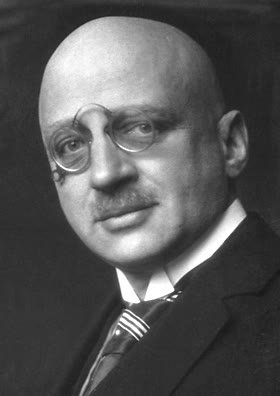
\includegraphics[width=\linewidth]{images/book2/haber.jpg}
\end{minipage}\hfill
\begin{minipage}[t]{0.78\linewidth}\vspace{0pt}
بيّن فريتس هابر أنه يمكن صنع الأمونيا من النيتروجين والهيدروجين
تحت الضغط على \omterm{def:b1:elementary-steps:catalyst}{حفّاز}؛ وحوّل كارل بوش التفاعل المخبري
إلى عملية صناعية. ونال هابر جائزة نوبل في الكيمياء
لعام 1918. والرجل نفسه أدار أول استعمال واسع النطاق للكلور
سلاحًا في الحرب العالمية الأولى: فالكيمياء التي تُطعم نصف البشرية
والكيمياء التي تقتل لا يفصل بينهما إلا اختيارات الكيميائيين.
(صورة: مؤسسة نوبل، نُشرت سنة 1919، ملكية عامة،
ويكيميديا كومنز.)
\end{minipage}
\end{history}

\section{الفوسفور والمنحيات نزولًا في الزمر}

الفوسفور، الواقع تحت النيتروجين، لا يكوّن روابط ثلاثية \ce{P#P}: فالفوسفور
الأبيض مكوّن من رباعيات أوجه \ce{P4}، مجهَدة ونشطة (إذ
يشتعل في الهواء ويُحفظ تحت الماء)؛ أما الفوسفور الأحمر فبوليمر،
أقل نشاطًا بكثير. واحتراق الفوسفور يعطي \ce{P4O10}، أشد الأكاسيد الشائعة
حمضيةً، الذي يعطي مع الماء حمض الفوسفوريك،
ذا قيم $\mathrm{p}K_a$ تساوي 2.15 و7.21 و12.34 (\cref{ch:b1:predominant-reaction}).
وصخر الفوسفات، المستخرج بنحو 250 مليون طن سنة 2025، يحوّله
حمض الكبريتيك إلى أسمدة فوسفاتية.
% ledger: usgs:phosphate-world-2025

نزولًا في كل \omterm{def:b1:periodicity:table}{زمرة} تصير العناصر أكثر فلزية (من البور إلى الثاليوم،
ومن الكربون إلى الرصاص، ومن النيتروجين إلى البزموت)، وأكاسيدها أكثر قاعدية،
وحالات الأكسدة الدنيا أكثر ثباتًا: وهذا \omterm{def:b1:p-block-13-15:inert-pair}{تأثير الزوج الخامل}. وعلى امتداد
\omterm{def:b1:periodicity:table}{الدورة}، تصير الأكاسيد أكثر حمضيةً، من \ce{Na2O} القاعدي إلى \omterm{def:b1:s-block:oxide-character}{الأكاسيد
الحمضية} للفوسفور والكبريت.

\section{تمارين}

\begin{exercise}[$\star$]\label{exo:b1:p-block-13-15:1}
أعطِ \omterm{def:b1:nernst:oxidation-number}{عدد أكسدة} النيتروجين في \ce{NH4NO3} (الذرتين كلتيهما)،
و\ce{N2O5}، و\ce{HNO2}، و\ce{N2H4} و\ce{Mg3N2}.
\end{exercise}

\begin{exercise}[$\star$]\label{exo:b1:p-block-13-15:2}
ارسم \omterm{def:b1:lewis-resonance-vsepr:lewis}{بنى لويس} للمركبات \ce{BF3} و\ce{NH3} والمركب الإضافي
\ce{F3B-NH3}؛ وعيّن \omterm{def:b1:lewis-resonance-vsepr:lewis-acid}{حمض لويس} وقاعدته.
\end{exercise}

\begin{exercise}[$\star$]\label{exo:b1:p-block-13-15:3}
اكتب تفاعلات \ce{CO2} و\ce{SiO2} (المنصهر) و\ce{P4O10} مع
هيدروكسيد الصوديوم، وتفاعلي \ce{Al2O3} مع حمض ومع قاعدة.
\end{exercise}

\begin{exercise}[$\star$]\label{exo:b1:p-block-13-15:4}
احسب ثابت توازن التفاعل \ce{N2 + 3H2 <=> 2NH3} عند
\qty{25}{\celsius} انطلاقًا من $\Delta_f G^\circ(\ce{NH3}) =
\qty{-16.45}{kJ/mol}$.
\end{exercise}

\begin{exercise}[$\star\star$]\label{exo:b1:p-block-13-15:5}
مستعملًا العدّ في \cref{prop:b1:p-block-13-15:silicate-units}، أعطِ
صيغة حلقة من ستة رباعيات أوجه يتقاسم كل منها رأسين (كما في البيريل)
وصيغة سلسلة مزدوجة يتقاسم فيها نصف رباعيات الأوجه رأسين
والنصف الآخر ثلاثة رؤوس.
\end{exercise}

\begin{exercise}[$\star\star$]\label{exo:b1:p-block-13-15:6}
احسب كتلة الألومينا المحصَّل عليها من طن واحد من بوكسيت يحتوي
\qty{55}{\percent} كتليًا من \ce{Al(OH)3}، بنسبة استرجاع قدرها \qty{92}{\percent}.
\end{exercise}

\begin{exercise}[$\star\star$]\label{exo:b1:p-block-13-15:7}
بيّن أن حمض البوريك \omterm{def:b1:lewis-resonance-vsepr:lewis-acid}{حمض لويس} لا \omterm{def:b1:predominant-reaction:bronsted}{حمض برونستد}،
وفسّر لماذا يكون محلوله حمضيًا مع ذلك.
\end{exercise}

\begin{exercise}[$\star\star$]\label{exo:b1:p-block-13-15:8}
وازن أكسدة الأمونيا إلى \ce{NO} \omterm{def:b1:nernst:oxidation-number}{بأعداد الأكسدة}
وأعطِ عدد الإلكترونات المتبادلة لكل \ce{NH3}.
\end{exercise}

\begin{exercise}[$\star\star$]\label{exo:b1:p-block-13-15:9}
تُصنع نترات الأمونيوم من الأمونيا وحمض النتريك. اكتب التفاعل،
واحسب كتلة الأمونيا اللازمة (لحمض النتريك وللمعادلة
معًا) لكل طن من نترات الأمونيوم.
\end{exercise}

\begin{exercise}[$\star\star\star$]\label{exo:b1:p-block-13-15:10}
فسّر لماذا كان النيتروجين غازًا ثنائي الذرة والفوسفور صلبًا من جزيئات \ce{P4}،
ولماذا كان ثنائي أكسيد الكربون غازًا والسيليكا صلبًا، مستعملًا
قوة روابط $\pi$ بين ذرات \omterm{def:b1:periodicity:table}{الدورة} الثانية وذرات \omterm{def:b1:periodicity:table}{الدورة} الثالثة.
\end{exercise}

\begin{exercise}[$\star\star\star$]\label{exo:b1:p-block-13-15:11}
بيّن \omterm{def:b1:nernst:electrode-potential}{بالجهود المعيارية} أن أكسيد الرصاص(IV) يؤكسد أيونات الكلوريد
إلى كلور في الوسط الحمضي، بينما لا يفعل أكسيد السيليكون(IV) شيئًا من هذا
القبيل. واربط ذلك \omterm{def:b1:p-block-13-15:inert-pair}{بتأثير الزوج الخامل}.
\end{exercise}

\begin{exercise}[$\star\star\star$]\label{exo:b1:p-block-13-15:12}
أنتج العالم نحو 160 مليون طن من النيتروجين على هيئة أمونيا سنة 2025.
فما كتلة الأمونيا الموافقة، وما كتلة الهيدروجين التي احتوتها؟
ومن أين يأتي ذلك الهيدروجين أساسًا؟
\end{exercise}

\section{مسألة: من الهواء إلى السماد}

\begin{problem}[{مسألة نهاية الأسبوع --- الرابطة الثلاثية للنيتروجين، وتخليق
الأمونيا، والخطوات الثلاث لصناعة حمض النتريك، ونترات الأمونيوم،
وكتلة حمض النتريك الممكن الحصول عليها من طن واحد من الأمونيا}]
\label{pb:b1:p-block-13-15:1}
يحوّل مصنع أسمدة الأمونيا إلى حمض نتريك وإلى نترات
الأمونيوم. الكتل المولية (\unit{g/mol}): \ce{N2} 28.0، \ce{H2} 2.0، \ce{NH3}
17.0، \ce{HNO3} 63.0، \ce{NH4NO3} 80.0، \ce{O2} 32.0؛
$\Delta_f G^\circ(\ce{NH3(g)}) = \qty{-16.45}{kJ/mol}$ عند
\qty{25}{\celsius}.

\medskip
\noindent\textbf{الجزء الأول --- النيتروجين.}
\begin{enumerate}
  \item ارسم \omterm{def:b1:lewis-resonance-vsepr:lewis}{بنية لويس} للجزيء \ce{N2} وبيّن لماذا هو خامل.
  \item أعطِ \omterm{def:b1:nernst:oxidation-number}{عدد أكسدة} N في \ce{N2} و\ce{NH3} و\ce{NO}
        و\ce{NO2} و\ce{HNO3} و\ce{NH4NO3}.
  \item اذكر ثلاث طرائق طبيعية أو صناعية \omterm{def:b1:p-block-13-15:nitrogen-fixation}{لتثبيت النيتروجين}.
  \item لماذا لا تستطيع النباتات استعمال \ce{N2} مباشرة؟
  \item أي عنصر يتأكسد وأيها يُختزل في تخليق
        الأمونيا؟
  \item اكتب تخليق الأمونيا.
\end{enumerate}

\medskip
\noindent\textbf{الجزء الثاني --- الأمونيا.}
\begin{enumerate}[resume]
  \item احسب ثابت توازن التخليق عند
        \qty{25}{\celsius}.
  \item لماذا يُجرى التخليق مع ذلك ساخنًا، على \omterm{def:b1:elementary-steps:catalyst}{حفّاز}؟
  \item احسب كتلتي \ce{N2} و\ce{H2} اللازمتين لطن واحد من
        الأمونيا.
  \item ما حجم الهواء (\qty{78}{\percent} \ce{N2} حجميًا، غاز
        مثالي، \qty{25}{\celsius}، \qty{1}{bar}) الذي يحتوي ذلك النيتروجين؟
  \item من أين يأتي الهيدروجين؟
  \item لماذا تُستعمل الأمونيا نفسها سمادًا في بعض البلدان،
        ولماذا كثيرًا ما تُحوَّل أولًا؟
\end{enumerate}

\medskip
\noindent\textbf{الجزء الثالث --- حمض النتريك.}
\begin{enumerate}[resume]
  \item وازن الخطوة 1، \ce{NH3 + O2 -> NO + H2O}، \omterm{def:b1:nernst:oxidation-number}{بأعداد الأكسدة}. % ce-unbalanced-ok
  \item وازن الخطوة 2، \ce{NO + O2 -> NO2}. % ce-unbalanced-ok
  \item وازن الخطوة 3، \ce{NO2 + H2O -> HNO3 + NO}. وأي نوع من تفاعلات الأكسدة % ce-unbalanced-ok
        والاختزال هو؟
  \item اجمع الخطوات مع إعادة تدوير كاملة لأحادي أكسيد النيتروجين NO في المعادلة
        الإجمالية.
  \item احسب كتلة الأكسجين المستهلكة لكل طن من الأمونيا.
  \item لماذا تُستعمل شبكة من البلاتين--الروديوم في الخطوة 1؟
\end{enumerate}

\medskip
\noindent\textbf{الجزء الرابع --- نترات الأمونيوم وحصائل الكتلة.}
\begin{enumerate}[resume]
  \item اكتب تكوّن نترات الأمونيوم.
  \item ما كسر الأمونيا الذي يجب تحويله إلى حمض نتريك
        لصنع نترات الأمونيوم وحدها؟
  \item احسب كتلة نترات الأمونيوم من طن واحد من الأمونيا
        موزَّع على هذا النحو.
  \item ما النسبة المئوية للنيتروجين في نترات الأمونيوم؟
  \item لماذا يجب تخزين نترات الأمونيوم بعيدًا عن المحروقات والحرارة؟
  \item احسب كتلة حمض النتريك الممكن الحصول عليها من طن واحد من
        الأمونيا (تحول تام).
\end{enumerate}
\end{problem}
